\scanpage{59}

Ce qui donne des conditions suffisantes pour la validité de c).
Cependant, elles ne sont pas nécessaires [même en exigeant la validité de c
pour $i<n$, et tous les tordus de $F$], comme on voit en faisant $n=1$:
car il suffit qu'on ait $\operatorname{prof}F_x\geq2$ pour $x$ fermé en $U$,
pour pouvoir conclure que
\[
H^0(U,F)\unsure{\mathbin{-}|\longrightarrow}H^0(\hat X,\hat F)
\]
est bijectif.

\figure{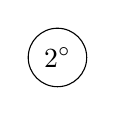
\begin{tikzpicture}\node[draw,circle] {$2^\circ$};\end{tikzpicture}}
La suite exacte nous apprend que \unsure{l'hom.}
\[
H^i(U,F)\longrightarrow H^{i+1}_Z(X,F)
\]
est un isom mod \unsure{vectoriels} finis. donc

\deleted{$H^i(U,F$}

\diagram{\begin{tikzpicture}
\node[anchor=north west,inner sep=0pt] (g) at (0,0) {\begin{tikzcd}[row sep=large]
H^i(U,F)\text{ de dim finie sur }k\arrow[d,Leftrightarrow]\\
H^{i+1}_z(F_z)\text{ de dim finie (i.e. de long. \unsure{finie}]}\quad
\text{pour }\forall\ z\in Z\arrow[d,Leftrightarrow]\\
z\unsure{\in}Z\Longrightarrow z\text{ pt isolé de }\operatorname{supp}E^{r-i-1}\cup\{z\}
\arrow[d,Leftrightarrow]\\
\alpha_{i+1}\text{ injectif pour }m\text{ grand}\arrow[d,Leftrightarrow]\\
H^i(X,F(m))\mathbin{-}H^i(U,F(\unsure{m|-m}))\quad\text{surjectif pour }m\text{ grand}
\end{tikzcd}};
\draw (g.north west) .. controls +(-.4,0) and +(-.2,.4) .. (g.west)
 .. controls +(-.2,-.4) and +(-.4,0) .. (g.south west);
\node[draw,circle] at (-1,-2.7) {$A'_i$};
\end{tikzpicture}}

\margin{58}
